\documentclass[tikz,border=8pt]{standalone}
% Shared look for every TikZ diagram. Load with \input{../../tools/tikz-style.tex}
\usepackage[sfdefault]{roboto}
\usetikzlibrary{arrows.meta, positioning, shapes.geometric, calc, fit, backgrounds}
\definecolor{cblue}{HTML}{4C78A8}
\definecolor{corange}{HTML}{F58518}
\definecolor{cgreen}{HTML}{54A24B}
\definecolor{cred}{HTML}{E45756}
\definecolor{cpurple}{HTML}{B279A2}
\definecolor{cgrey}{HTML}{6B6B6B}
\tikzset{
  every picture/.style={font=\sffamily, line width=1.2pt},
  box/.style={draw=#1, fill=#1!12, rounded corners=4pt, align=center, inner sep=7pt, minimum height=1.1cm},
  box/.default=cgrey,
  arrow/.style={-{Stealth[length=3mm]}, draw=cgrey, line width=1.4pt},
  title/.style={font=\sffamily\bfseries\Large},
  note/.style={font=\sffamily\small, text=cgrey, align=center},
}
\AtBeginDocument{\hyphenpenalty=10000 \exhyphenpenalty=10000}

% Autoware Universe lane driving (autoware_launch param files, 2026-10): behavior_path_planner 300 m, points every
% 2 m, 10 Hz; elastic_band_smoother 100 points x 1 m, clearance 0.1 m, OSQP; path_optimizer (MPT) 100 x 1 m, OSQP;
% velocity_smoother (JerkFiltered) 200 m, OSQP. All re-solve on every new input.
\begin{document}
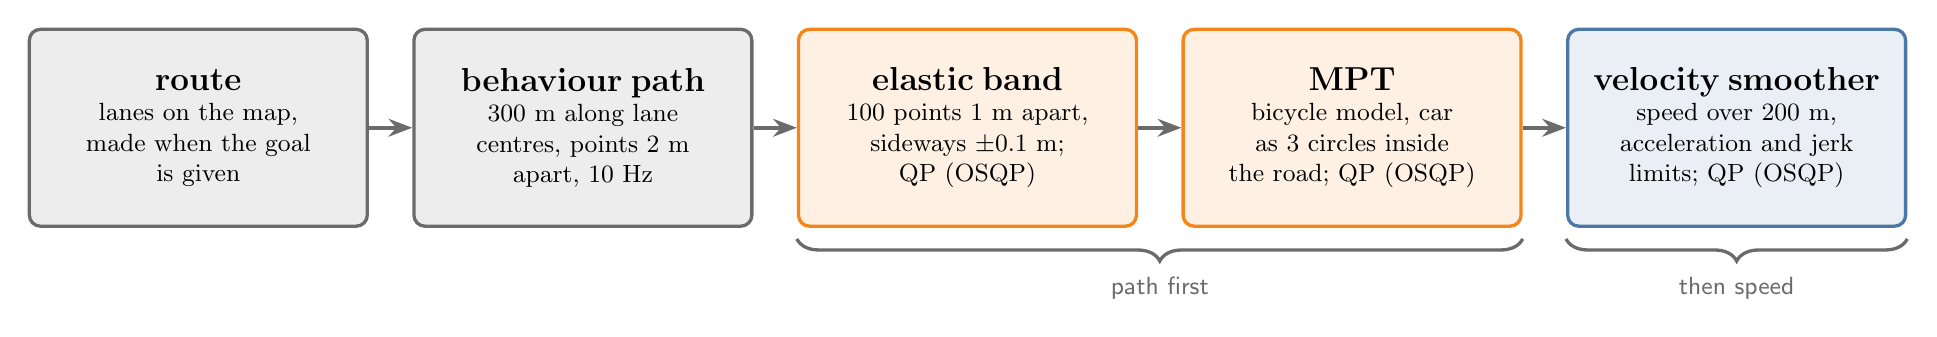
\begin{tikzpicture}[node distance=0.55cm,
  st/.style={box=#1, font=\small, minimum width=4.1cm, text width=3.8cm, minimum height=2.5cm}]
  \node[st=cgrey] (a) {{\large\textbf{route}}\\ lanes on the map,\\ made when the goal\\ is given};
  \node[st=cgrey, right=of a] (b) {{\large\textbf{behaviour path}}\\ 300 m along lane\\ centres, points 2 m\\ apart, 10 Hz};
  \node[st=corange, right=of b] (c) {{\large\textbf{elastic band}}\\ 100 points 1 m apart,\\ sideways $\pm$0.1 m;\\ QP (OSQP)};
  \node[st=corange, right=of c] (d) {{\large\textbf{MPT}}\\ bicycle model, car\\ as 3 circles inside\\ the road; QP (OSQP)};
  \node[st=cblue, right=of d] (e) {{\large\textbf{velocity smoother}}\\ speed over 200 m,\\ acceleration and jerk\\ limits; QP (OSQP)};
  \draw[arrow] (a) -- (b); \draw[arrow] (b) -- (c); \draw[arrow] (c) -- (d); \draw[arrow] (d) -- (e);
  \draw[decorate, decoration={brace, amplitude=8pt, mirror}, draw=cgrey] ([yshift=-4pt]c.south west) -- node[note, below=10pt] {path first} ([yshift=-4pt]d.south east);
  \draw[decorate, decoration={brace, amplitude=8pt, mirror}, draw=cgrey] ([yshift=-4pt]e.south west) -- node[note, below=10pt] {then speed} ([yshift=-4pt]e.south east);
\end{tikzpicture}
\end{document}
